\documentclass[11pt,a4paper]{article}

\usepackage[colorlinks=true,linkcolor=blue,urlcolor=blue,citecolor={blue}]{hyperref}
\usepackage{epsfig,amssymb}
\usepackage{hyperref}
\usepackage[latin1]{inputenc}
\usepackage[english]{babel}
\usepackage{lscape} % for having landscape page
\usepackage[numbers]{natbib} % biblography
\usepackage{datetime} % only month and year
\usepackage{amsmath}
\usepackage{listings} % source code
\usepackage{graphicx} %picture
\usepackage{float}
\usepackage{comment}
\usepackage{caption}
\usepackage[table]{xcolor}
\usepackage{program}
\usepackage{fancyhdr}
\usepackage{lastpage}
\usepackage{tabularx}

\floatstyle{ruled}
\newfloat{program}{thp}{lop}
\floatname{program}{Code}
\captionsetup [program]{labelsep = colon}


\hypersetup{
    colorlinks=true,       % false: boxed links; true: colored links
    linkcolor=blue,          % color of internal links
    citecolor=blue,        % color of links to bibliography
    urlcolor=blue           % color of external links
}


\pagestyle{plain}
\newcommand{\horiz}{{\rule{\textwidth}{.5pt}}}
\renewcommand{\baselinestretch}{1.0}

\renewcommand{\today}{\ifcase\month\or
   January\or February\or March\or April\or May\or June\or
   July\or August\or September\or October\or November\or December\fi
   \space\number\year}

\title{\Large \bf SD Erlang Version of Orbit}

\author{ Amir Ghaffari, Natalia Chechina, Phil Trinder
\\The School of Computing Science
\\  Glasgow University
\\Glasgow, G12 8QQ, UK}

\begin{document}
\maketitle
\thispagestyle{empty}
%\clearpage
%\tableofcontents
\thispagestyle{empty}
%\clearpage
\setcounter{page}{1}

\pagestyle{fancy}
\rhead{\footnotesize \parbox{11cm}{} }


\section{Orbit Calculations}

An $Orbit$ is a symbolic computing kernel and is a generalization of a transitive closure computation\cite{Lubeck2001}. To compute $Orbit$ for a given space $[0..X]$  a list of generators $g1, g2,..., gn$ are applied on an initial vertex $x_{0}\in [0..X]$.  This will create new numbers $(x_{1}...x_{n}) \in [0..X]$. Repeatedly, generator functions are applied on each of the new numbers and this continues until no new number is generated.

\section{Distributed Erlang Orbit}

Orbit computation is initiated by a master process. Master establishes a P2P network of worker processes on available nodes. Each worker process owns part of a distributed hash table. A hash function is applied on a generated number to find to which worker it belongs.

To detect the termination of Orbit computation, a credit/recovery distributed algorithm is used \cite{Matocha1998}. Initially the master process has a specific amount of credit. Each active process holds a portion of the credit and when a process becomes passive, i.e. the process become inactive for for a specific period of time, it sends the credit it holds to active processes. When master process collects all the credit, it detects that termination has occurred.

Distributed Erlang Orbit has a flat design in which all nodes are fully connected. As shown in Figure~\ref{fig:flat_design}, master process initiates Orbit computation on all worker nodes and each worker node has connections to the other worker nodes.

The following features in Orbit makes the benchmark a desirable case study for SD Erlang:
\begin{itemize}
  \item It uses a Distributed Hash Table (DHT) similar to NoSQL DBMS like Riak that use replicated DHTs \cite{BashoConcepts2013}.
  \item It uses standard P2P techniques and credit/recovery distributed termination detection algorithm.
  \item It is only a few hundred lines and has a  good performance and extensibility.
\end{itemize}

\begin{figure}[h]
    \centering
    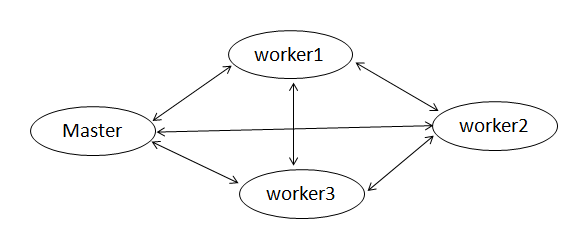
\includegraphics  [ keepaspectratio, width=80mm]  {./img/flat_design.png}
    \caption{Communication Model in Distributed Erlang Orbit}
    \label{fig:flat_design}
\end{figure}

\section{Scalable Distributed  Erlang Orbit}

\subsection*{Communication Model}
 To reduce the number of connections, we propose a new design for Orbit in which nodes are grouped into sets of s\_groups. In SD-Erlang, s\_group nodes have transitive connections with the nodes from the same s\_group, and non-transitive connections with other nodes.

\begin{figure}[h]
    \centering
    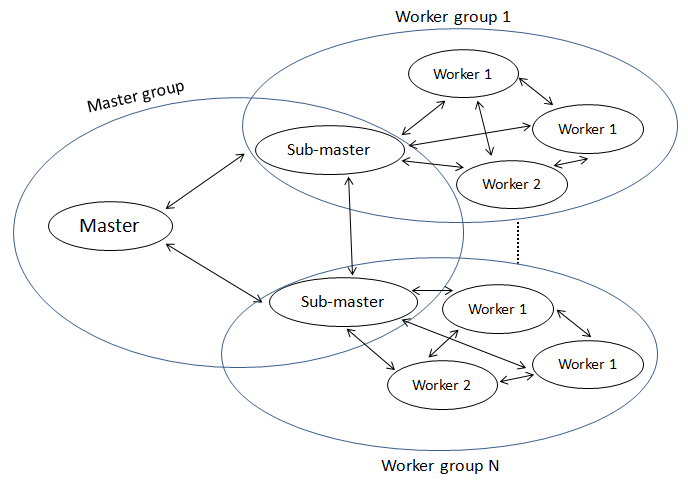
\includegraphics  [ keepaspectratio, width=80mm]  {./img/sd_design.png}
    \caption{Communication Model in SD Erlang Orbit}
    \label{fig:sd_design}
\end{figure}

As shown in Figure~\ref{fig:sd_design}, there are two kind of s\_groups in this model: ~\texttt{master} and ~\texttt{worker}. There is just one ~\texttt{master} s\_group that master node and all the sub-master nodes belong to it. There can be multiple~\texttt{worker} s\_groups in the system. Each ~\texttt{worker} s\_group has just one sub-master node and an arbitrary number of worker nodes.

Communication between nodes inside an s\_group in done directly but when a worker node needs to communicate with another worker node outside its own s\_group, communication is done through sub-master nodes. In this case, the number of messages increases three times, i.e. assume A and C belong to different s\_groups, so instead of sending a message from A to C directly (A$\rightarrow$C), we would have: A$\rightarrow A_{submaster}\rightarrow C_{submaster}\rightarrow$C. 

This approach reduces the number of connections between nodes. The  number of connections on a worker node is equal to the size of s\_group and the number of connections on a sub-master node is equal to the number of worker nodes inside the s\_group \emph{plus} the number of all the other sub-master nodes, i.e.
\begin{itemize}
\item The number of connections of a worker node is equal to the size of s\_group 
\item The number of connections of a sub-master node is equal to the number of worker nodes inside the group \emph{plus} the number of all the other sub-master nodes
\end{itemize}

\subsection*{Computation Model}

The Orbit computation is started by master process on the master node. Master process dynamically and evenly divides  nodes to a number of s\_groups. After creating s\_groups, the first node of each s\_group is chosen as sub-master node. Then, master process runs two processes, i.e. ~\texttt{submaster} and ~\texttt{gateway}, on each sub-master node. A submaster process is responsible to initiate, collect credits and data, and terminate the worker processes in its own s\_group and send the collected data back to the master process. In other words, a submaster process is master's representative in an s\_group and behaves like an interface between master and worker processes.

The another process on a sub-master node is ~\texttt{gateway}. When two worker processes from two different s\_groups need to communicate, the gateway processes of both s\_groups participate as follow:

Assume ~\texttt{Process1} from ~\texttt{s\_group1} needs to send a message to ~\texttt{process2} in ~\texttt{s\_group2}. The name of gateway processes are ~\texttt{gateway1} and ~\texttt{gateway2} in ~\texttt{s\_group1} and ~\texttt{s\_group2} respectively. The message path would be: ~\texttt{Process1}$\rightarrow$~\texttt{gateway1}$\rightarrow$~\texttt{gateway2}$\rightarrow$~\texttt{process2}. 

\subsection*{Double Hashing} In distributed Erlang Orbit, all processes store a copy of hash table that specifies which process is responsible for which fragment of the hash table. However, in SD Erlang design, there are two levels of hash tables. The first level hash table that is created by master process and stored on all sub-master processes, specifies which group is responsible for which part of the table. The second level hash table is created by sub-masters and stored on worker processes. Each worker process stores a table that specifies which process in the s\_group is responsible for which part of the table. For example Table \ref{tab:group_hash_table} shows how range 1-300 is divided among three groups. In Table \ref{tab:processes_hash_table} it is depicted that how Group1 is divided among 4 processes equally.

\begin{table}
\parbox{.45\linewidth}{
\centering

\begin{tabular}{ | c | l | }
	\hline
	Group1 & 1-100 \\ \hline
	Group2 & 101-200 \\ \hline
	Group3 & 201-300 \\ \hline
	\end{tabular}

	\caption{Group Hash Partition}
	\label{tab:group_hash_table}
}
\hfill
\parbox{.60\linewidth}{
\centering

\begin{tabular}{ | c | l | }
	\hline
	Process1 & 1-25 \\ \hline
	Process2 & 26-50 \\ \hline
	Process3 & 51-75 \\ \hline
	Process4 & 76-100 \\ \hline
	\end{tabular}

	\caption{Process Table Partition within Group 1}
	\label{tab:processes_hash_table}
}
\end{table}

\section{Code structure}

This section lists all the modules in SD Erlang Orbit with a brief explanation.

\subsection*{grouping.erl}
The grouping module contains functions that dynamically create the s\_groups.
\begin{itemize}
\item it creates an s\_group for the master and all sub-master nodes in function ~\texttt{create\_group\_list}
\item it creates an s\_group for a sub-master and all its worker nodes in function ~\texttt{make\_group}
\item the Orbit space is divided among s\_groups in function ~\texttt{create\_group\_list}
\end{itemize}

\subsection*{init\_bench.erl}
Initial value for computing Orbit such as number of processes on each worker node, number of s\_groups, and the size of s\_groups are set in the main function.

\subsection*{bench.erl}
Generator functions and a function for distributed computation are in the module.

\subsection*{worker.erl}
All functions related to a worker process such as receiving a vertex, generating new vertexes, and forwarding them to appropriate gateways are in this module.

\subsection*{master.erl}
The module creates groups hash table, sub-master processes, gateway processes, and distributes the groups hash table among gateway processes. Collecting credits and the Orbit data also is done in this module.

\subsection*{sub\_master.erl}
A sub-master process initiates all the worker processes inside its own s\_group and collects their credits and data. Gateway process which handles communication between s\_groups, is defined in this module as well.

\subsection*{credit.erl}
Termination algorithm based on credit/recovery is implemented in this module. 

\subsection*{table.erl}
The module implemented a hash tables which has a fixed number of slots but each slot can store a list of vertices. 

\subsection*{config.erl}
Load the configuration file and provides a function for reading the value of a key. 

\bibliographystyle{unsrtnat}
\bibliography{bibliography}

\end{document}
